%\documentclass[dvipdfmx]{beamer}      % platex の場合
\documentclass[handout]{beamer}        % lualatex の場合
\usepackage{mySld}

\begin{document}
\title{基礎コンピュータ工学\\第3章 組み立て\\
       (パート2:ハンダ付け2)}
\date{}

\begin{frame}
  \titlepage
  \centerline{\url{https://github.com/tctsigemura/TecTextBook}}
  \vfill
  \centerline{本スライドの入手:
    \raisebox{-7mm}{\includegraphics[scale=0.3]{../Img/QRs3_2.png}}}
\end{frame}

%==============================================================================
%\begin{frame}
%  \frametitle
%  \tableofcontents
%\end{frame}

\section{組み立て}
%==============================================================================
\begin{frame}
  \frametitle{IC(1)}
  \vfill
  \centerline{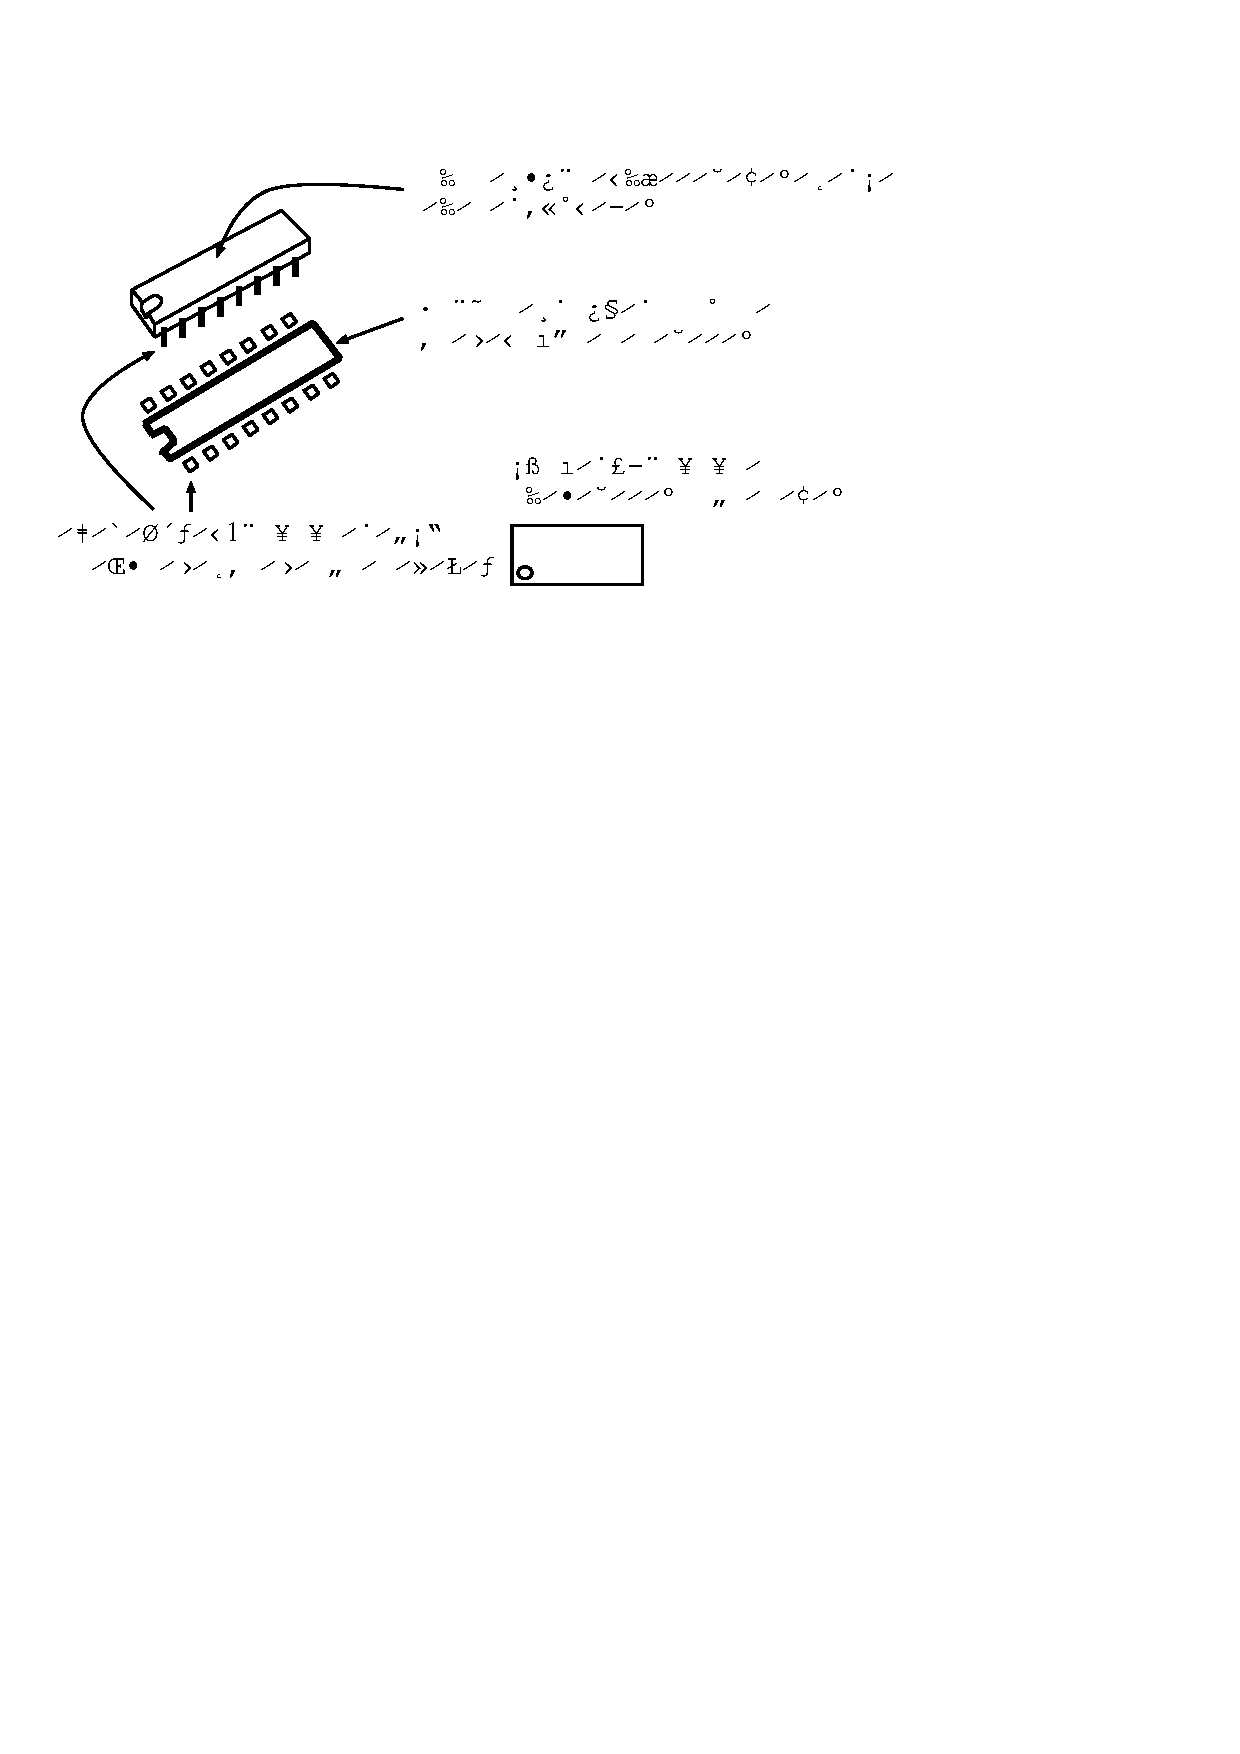
\includegraphics[scale=0.65]{../chap3/ic.pdf}}
  \vfill
  \centerline{\small\begin{tabular}{l|l|l}
    \hline
    \hline
    \multicolumn{1}{c|}{記号} &
    \multicolumn{1}{c|}{型番} &
    \multicolumn{1}{c}{説明} \\
    \hline
    U3 & K516       & 水晶発振 IC \\
    U6 & LM339      & 電圧比較 IC \\
  \end{tabular}}
\end{frame}

%==============================================================================
\begin{frame}
  \frametitle{IC(2)}
  \vfill
  \centerline{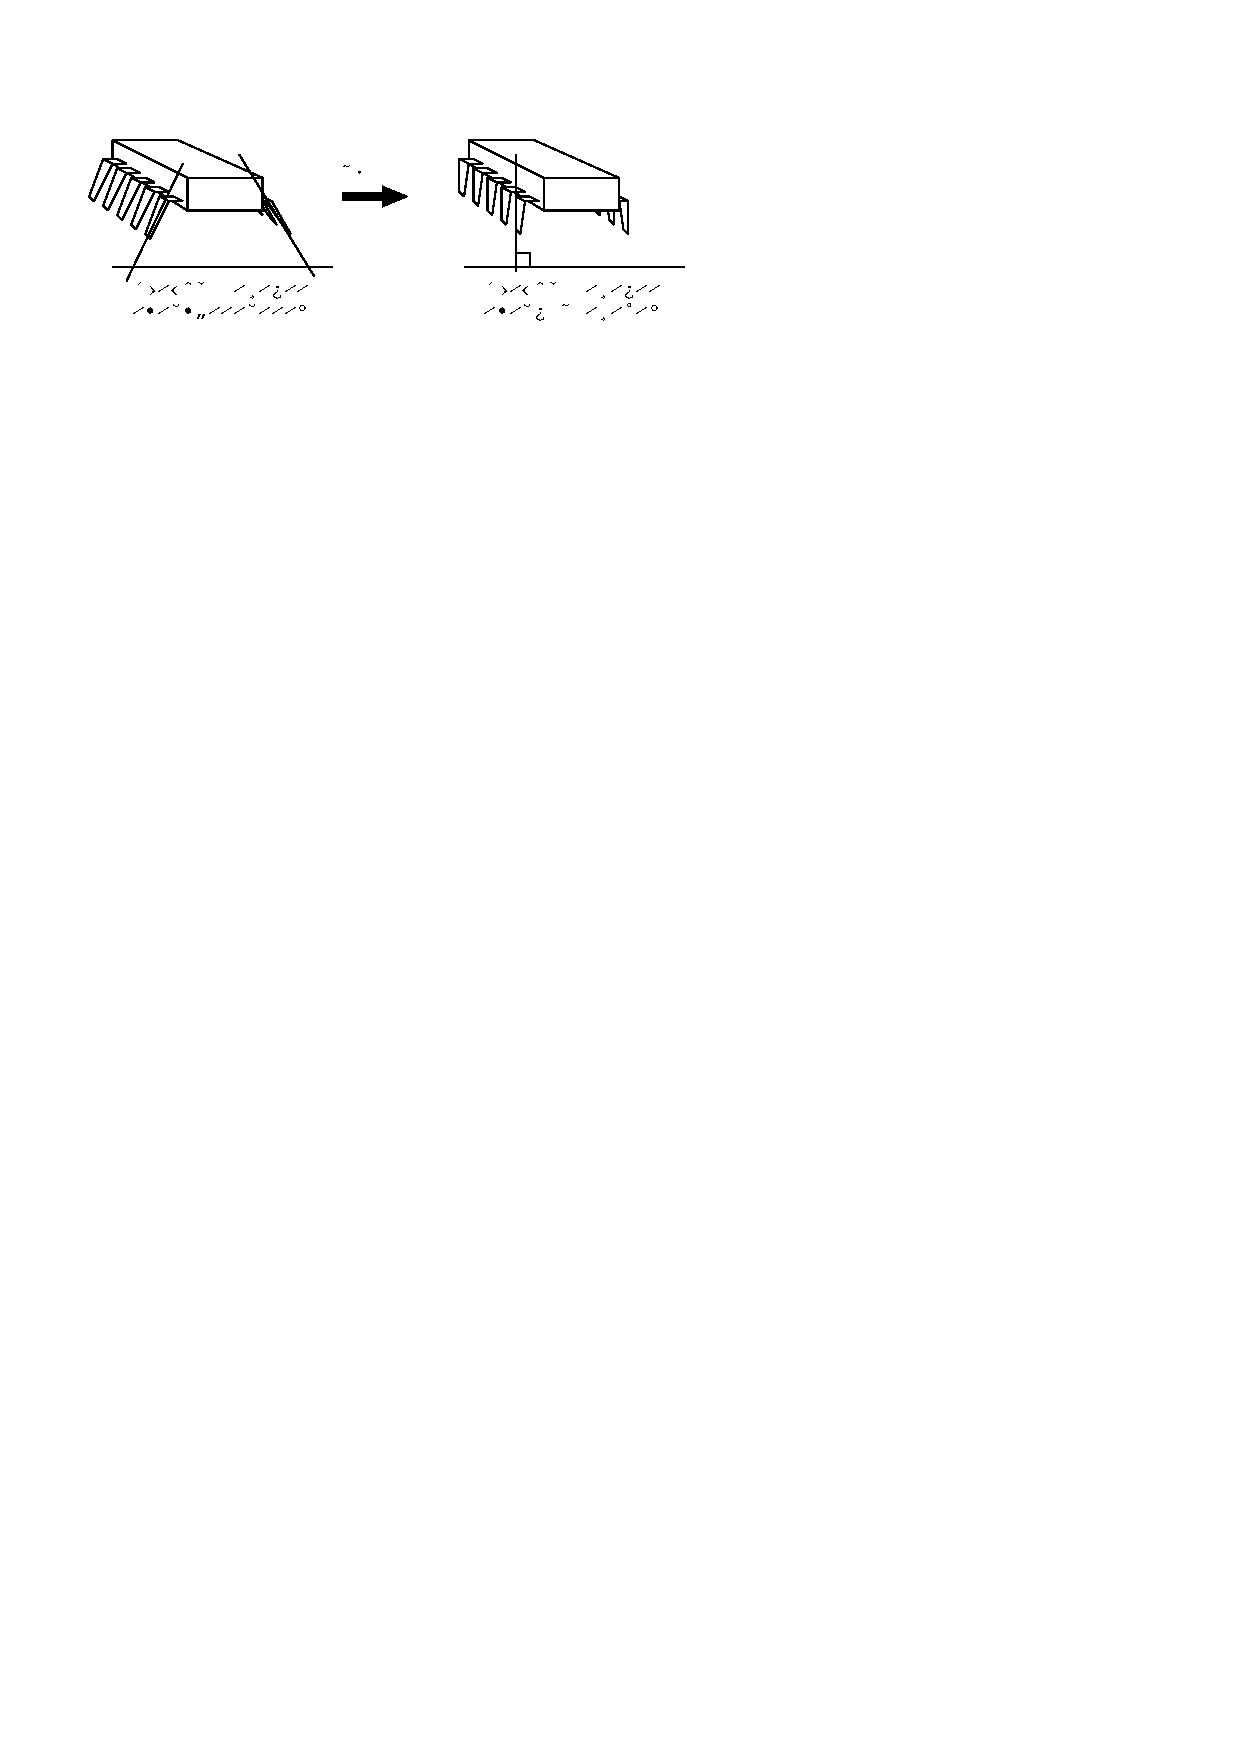
\includegraphics[scale=0.8]{../chap3/icnoasi.pdf}}
  \vfill
  \begin{itemize}
  \item ICには向きがあるので注意!!
  \item 足が基板に垂直になるように手直しする.(動画を参考に)
  \item 対角線上の二箇所を仮のハンダ付けする.\\
    → 浮き上がりは,まだ,修正できる.\\
    → 向きを間違っている場合は先生に頼む.
  \item 三つ以上の足をハンダ付けしたあとでは修正が難しい.
  \end{itemize}
\end{frame}

%==============================================================================
\begin{frame}
  \frametitle{フェライトビーズ}
  \centerline{\includegraphics[scale=0.9]{../Tikz/bead.pdf}}
  \vfill
  \centerline{\small\begin{tabular}{l|l|l}
    \hline
    \hline
    \multicolumn{1}{c|}{記号} &
    \multicolumn{1}{c|}{型番} &
    \multicolumn{1}{c}{説明} \\
    \hline
    FB1,2 & なし & なし \\
  \end{tabular}}
  \vfill
  \begin{itemize}
    \item 向きはない.
    \item やけどに注意!!
  \end{itemize}
\end{frame}

%==============================================================================
\begin{frame}
  \frametitle{}
  \begin{minipage}{0.55\columnwidth}
    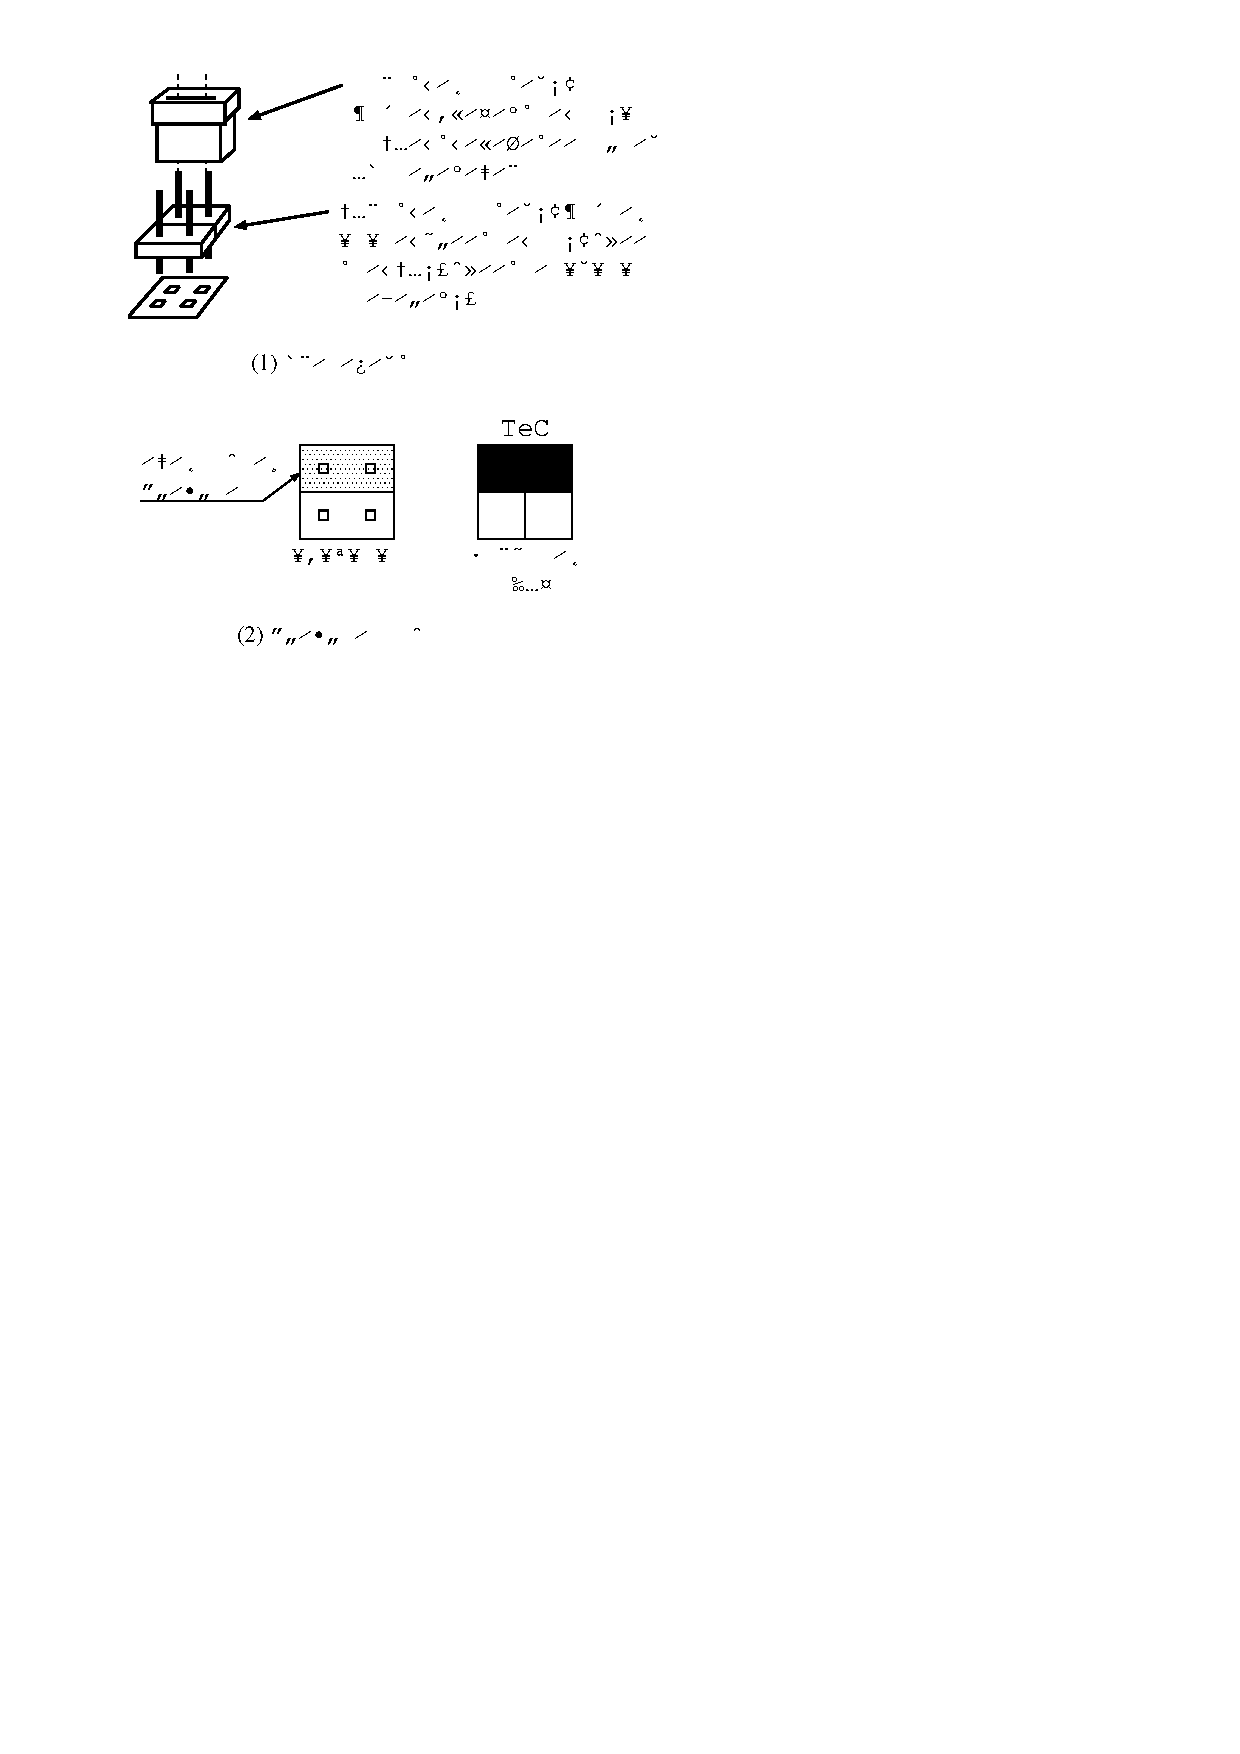
\includegraphics[scale=0.8]{../chap3/jp.pdf}
  \end{minipage}
  \begin{minipage}{0.44\columnwidth}
    \begin{center}
      {\small\begin{tabular}{l|l|l}
        \hline
        \hline
        \multicolumn{1}{c|}{記号} &
        \multicolumn{1}{c|}{型番} &
        \multicolumn{1}{c}{説明} \\
        \hline
        J1 & なし &  なし \\
        \end{tabular}}
    \end{center}
  \end{minipage}
\end{frame}

%==============================================================================
\begin{frame}
  \frametitle{圧電スピーカ}
  \centerline{\includegraphics[scale=0.8]{../Tikz/buz.pdf}}
  \vfill
  \centerline{\small\begin{tabular}{l|l|l}
    \hline
    \hline
    \multicolumn{1}{c|}{記号} &
    \multicolumn{1}{c|}{型番} &
    \multicolumn{1}{c}{説明} \\
    \hline
    BZ1 & なし & 圧電スピーカ \\
  \end{tabular}}
\end{frame}

%==============================================================================
\begin{frame}
  \frametitle{電解コンデンサ}
  \centerline{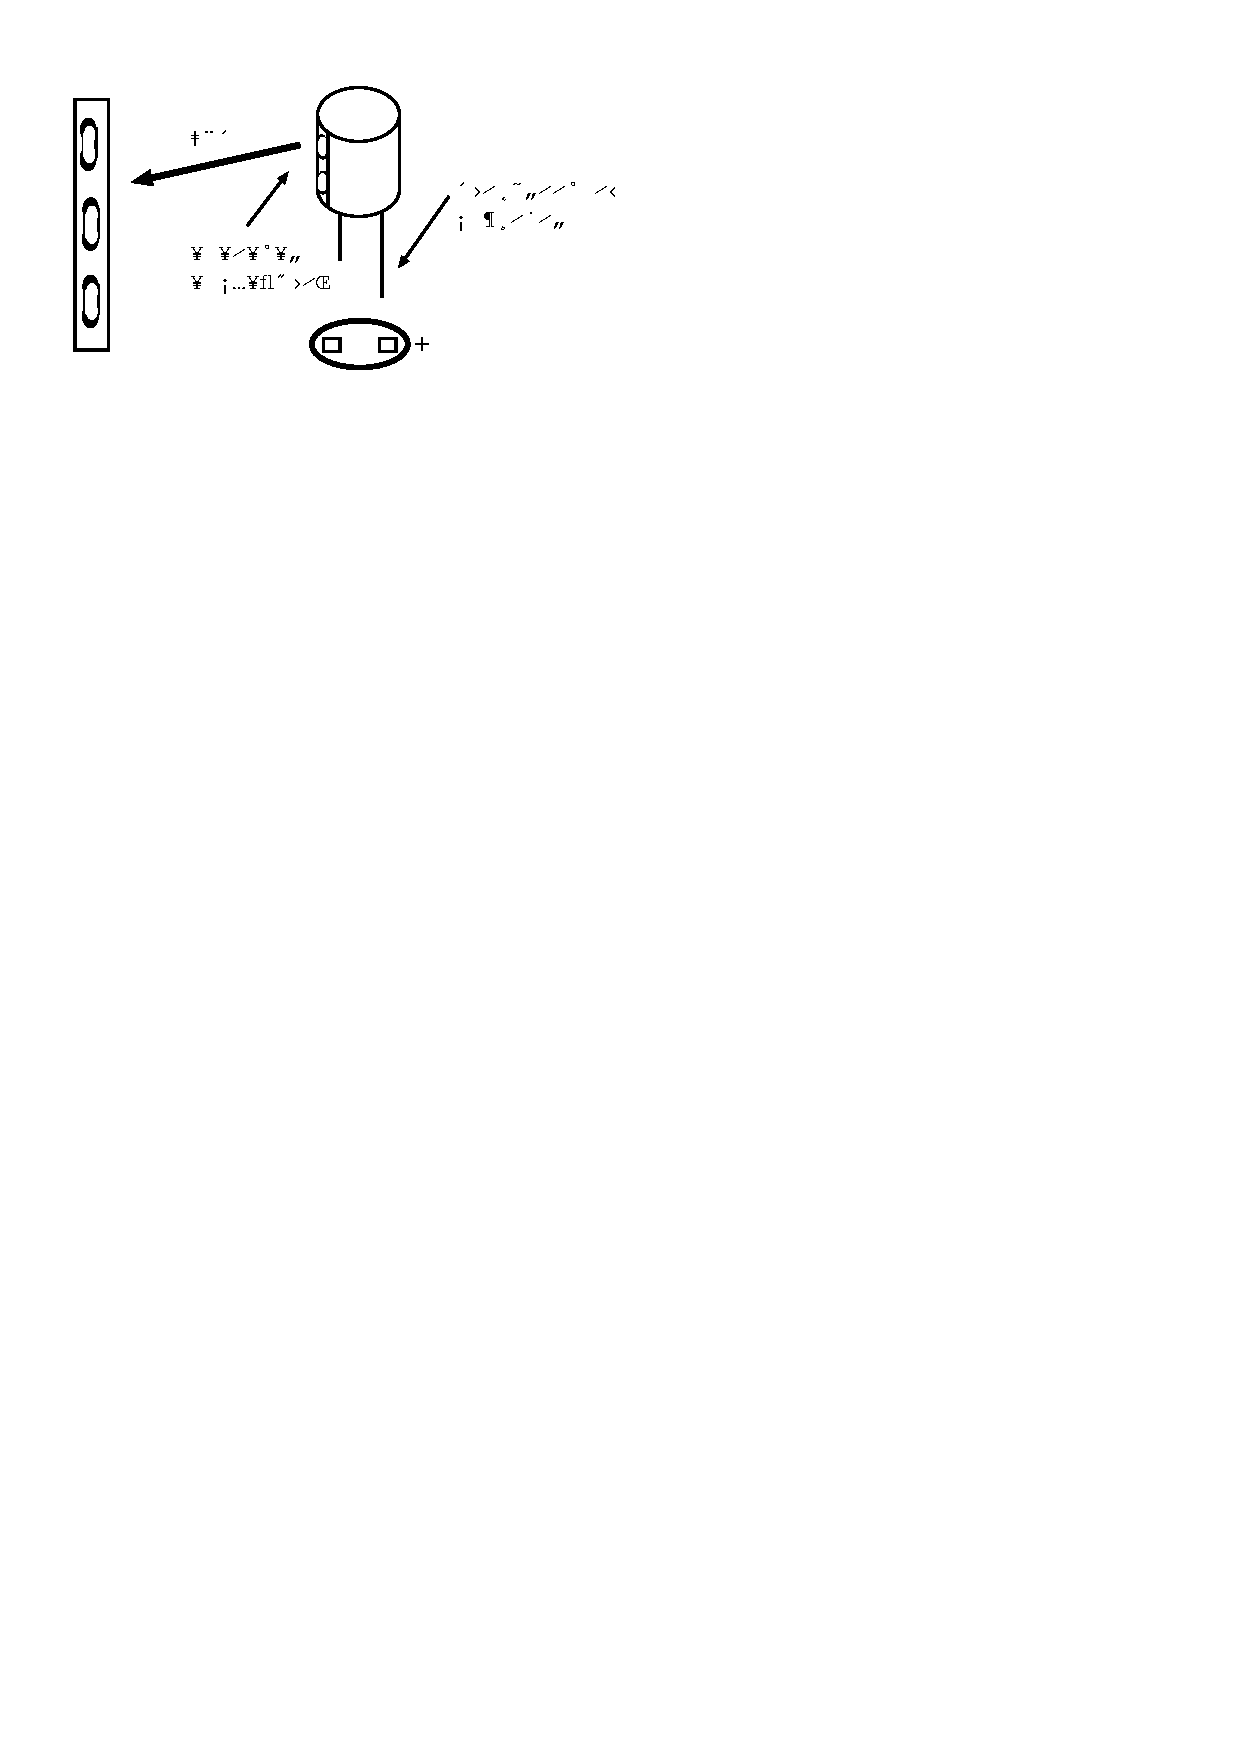
\includegraphics[scale=0.7]{../chap3/denkai.pdf}}
  \vfill
  \centerline{\small\begin{tabular}{l|l|l}
    \hline
    \hline
    \multicolumn{1}{c|}{記号} &
    \multicolumn{1}{c|}{型番} &
    \multicolumn{1}{c}{説明} \\
    \hline
    C0,C5,C7,C9,C16 & $ 25V 47 \mu F $ & $ 47 \mu F$ \\
    C11             & $ 10V 220 \mu F $ & $ 220 \mu F$ \\
  \end{tabular}}
  \vfill
  \begin{itemize}
  \item 向きがあるので注意!!
  \item 部品の浮き上がりに注意!!(やがて足が折れる)
  \end{itemize}
\end{frame}

%==============================================================================
\begin{frame}
  \frametitle{JTAGコネクタ}
  \centerline{\includegraphics[scale=1.2]{../Tikz/cn.pdf}}
  \vfill
  \centerline{\small\begin{tabular}{l|l|l}
      \hline
      \hline
      \multicolumn{1}{c|}{記号} &
      \multicolumn{1}{c|}{型番} &
      \multicolumn{1}{c}{説明} \\
      \hline
      CN4 & なし & 小さい14ピンのコネクタ \\
    \end{tabular}
  }
  \vfill
  \begin{enumerate}
  \item[1.] 向きに注意!!
  \item[2.] 中央付近の一本をハンダ付けする.
  \item[3.] 向き,傾きを再度確認する.
  \item[4.] 残りの足をハンダ付けする.
  \end{enumerate}
  \vfill
\end{frame}

%==============================================================================
\begin{frame}
  \frametitle{電源コネクタ}
  \centerline{\includegraphics[scale=0.65]{../Keynote/cn1-crop.pdf}}
  \vfill
  \centerline{\small\begin{tabular}{l|l|l}
    \hline
    \hline
    \multicolumn{1}{c|}{記号} &
    \multicolumn{1}{c|}{型番} &
    \multicolumn{1}{c}{説明} \\
    \hline
    CN1 & なし & USB-B コネクタ \\
  \end{tabular}}
  \vfill
  \emph{\Large\color{red}やけどに注意!!}
  \begin{enumerate}
  \item[1.] 穴にしっかり差し込む.
  \item[2.] 大きな穴とコネクタの端子を十分熱する.
  \item[3.] 大きな穴が塞がるまで,ハンダをどんどん融かし込む.
  \item[4.] \emph{十分に冷めるのを待つ.}
  \item[5.] 部品が傾いていないか確認する.
  \item[6.] 小さな穴に部品の足をハンダ付けする.
  \end{enumerate}
  \vfill
\end{frame}

%==============================================================================
%\begin{frame}
%  \frametitle{}
%\end{frame}

\end{document}
